 \chapter{Introduction}
\label{chap:introduction}

The invention of the optical frequency comb two decades ago initiated a revolution in precision measurement by dramatically improving the resolution with which we can conveniently measure time and frequency \cite{Diddams2000,Jones2000,Udem2002,Hall2006,Hansch2006}. This revolution was brought about by the realization of a simple scheme\footnote{that required markedly \textit{less} simple advancements in capabilities in nonlinear optics \cite{Ranka2000}.} by which the hundreds-of-terahertz-scale optical frequencies of a modelocked laser could be measured electronically, and was facilitated by the development of high performing solid-state femtosecond laser technology such as the Ti:sapphire laser. Optical frequency combs have found important roles in experiments and applications in contexts including the first demonstration of an optical atomic clock \cite{Diddams2001}, systems for ultra-low-noise microwave synthesis \cite{Fortier2011}, broadband spectroscopy applications \cite{Diddams2007,Coddington2016}, optical arbitrary waveform generation \cite{Cundiff2010}, and stable long-term calibration of astronomical spectrographs for exoplanet detection \cite{Steinmetz2008}. Further development of the technology beyond the first stabilization of the Ti:sapphire laser that heralded the frequency comb's arrival has enabled combs to reach applications across many wavelength bands \cite{Washburn2004a,Gohle2005b,Diddams2010,Faist2016}. The technology is reaching maturity, and frequency combs have been commercially available for some time.

In the last decade, methods for generating optical frequency combs without a modelocked laser have begun to suggest new ways to bring their capabilities to applications outside the controlled environment of the research laboratory. These new frequency combs come with higher repetition rates, and this makes them particularly attractive for applications where high power per comb mode, individual accessibility of comb modes, and fast acquisition times are desired. These applications include arbitrary microwave and optical waveform generation, telecommunications, and broadband, fast-acquisition-time spectroscopy. Moreover, these combs come with lower size, weight, and power (SWAP) requirements, which will enable them to bring the features that make modelocked-laser-based combs attractive into the field, enabling e.g. direct optical frequency synthesis on a chip \cite{Spencer2018}.

This thesis focuses on these new approaches for frequency comb generation. The bulk of the thesis covers microresonator-based frequency combs, and especially the nonlinear dynamics involved in the generation of these frequency combs via the Kerr nonlinearity; an introduction to this field is provided in Chapter \ref{chap:microresonators}. Chapters \ref{chap:PMPumping}-\ref{FPLLE} describe advancements in the field. Chapter \ref{chap:EOMCombs} presents a second method for generating a high-repetition-rate frequency comb without modelocking that is based on active modulation of a CW seed laser and subsequent nonlinear spectral broadening. In Chapter \ref{chap:PulsePicking}, I present experimental and theoretical investigations of repetition-rate reduction of frequency combs via pulse gating, which may prove useful for adapting low-SWAP combs and their intrinsically high repetition rates to some applications as the technology continues to develop. Finally, in Chapter \ref{chap:Conclusion} I discuss avenues for further research.

In the remainder of this chapter, I discuss the basic properties of frequency combs and explain how the optical frequencies making up a comb can be fully determined by electronics operating with gigahertz-scale bandwidths.

\section{Optical frequency combs}

An optical frequency comb is obtained by fully stabilizing the spectrum of an optical pulse train. The first frequency combs came about through full frequency-stabilization of modelocked lasers; this thesis focuses on frequency combs with pulse trains generated through other means.

\subsection{Optical pulse trains and their spectra}

In the time domain, a frequency comb consists of a train of uniformly spaced optical pulses arriving at the pulse train's repetition rate $f_{rep}$, which within the rapidly expanding space of frequency comb technology is between $\sim$10 MHz and $\sim$1 THz. These pulses are typically very short compared to their repetition period $T=1/f_{rep}$, with durations on the order of 100 fs. In the frequency domain, the comb consists of a set of modes that are spaced by $f_{rep}$ in frequency and that have amplitudes determined by an overall spectral envelope centered at the optical carrier frequency $\nu_c$ ($\sim$193 THz in this thesis), with bandwidth inversely related to the temporal duration of the pulses. The usual description of a frequency comb, which is natural for modelocked-laser-based combs that are not derived from a CW laser, gives the frequencies of these modes as 
\begin{equation}
\nu_n=nf_{rep}+f_0, \label{eq:combfreqsold}
\end{equation} 
where $n\sim \nu_c/f_{rep}$ for the optical modes that make up the comb and $f_0$ is the carrier-envelope offset frequency, which may be defined to be between $0$ and $f_{rep}$. The offset frequency results from the pulse-to-pulse evolution of the carrier wave underneath the temporal intensity envelope of the pulses due to a difference in group and phase velocities. An equivalent representation of the frequencies of the comb that is more natural for frequency combs directly derived from a CW laser, as described in this thesis, is
\begin{equation}
\nu_\mu=\nu_c+\mu f_{rep}, \label{eq:combfreqsnew}
\end{equation} 
where $\nu_c$ is the frequency of the CW laser, the `pump' or `seed' laser, from which the frequency comb is derived and $\mu$ is a pump-referenced mode number, in contrast with the zero-referenced mode number $n$ of Eq. \ref{eq:combfreqsold}. Now the carrier-envelope offset frequency $f_0$ is found in the difference between $\nu_c$ and the closest harmonic of $f_{rep}$: $f_0=\nu_c-N f_{rep}$, where $N$ is the largest integer such that $f_0>0$. Fig. \ref{fig:CombBasics} depicts the properties of a frequency comb in the time domain and the frequency domain.

\begin{figure}[htpb]
	\begin{center}
		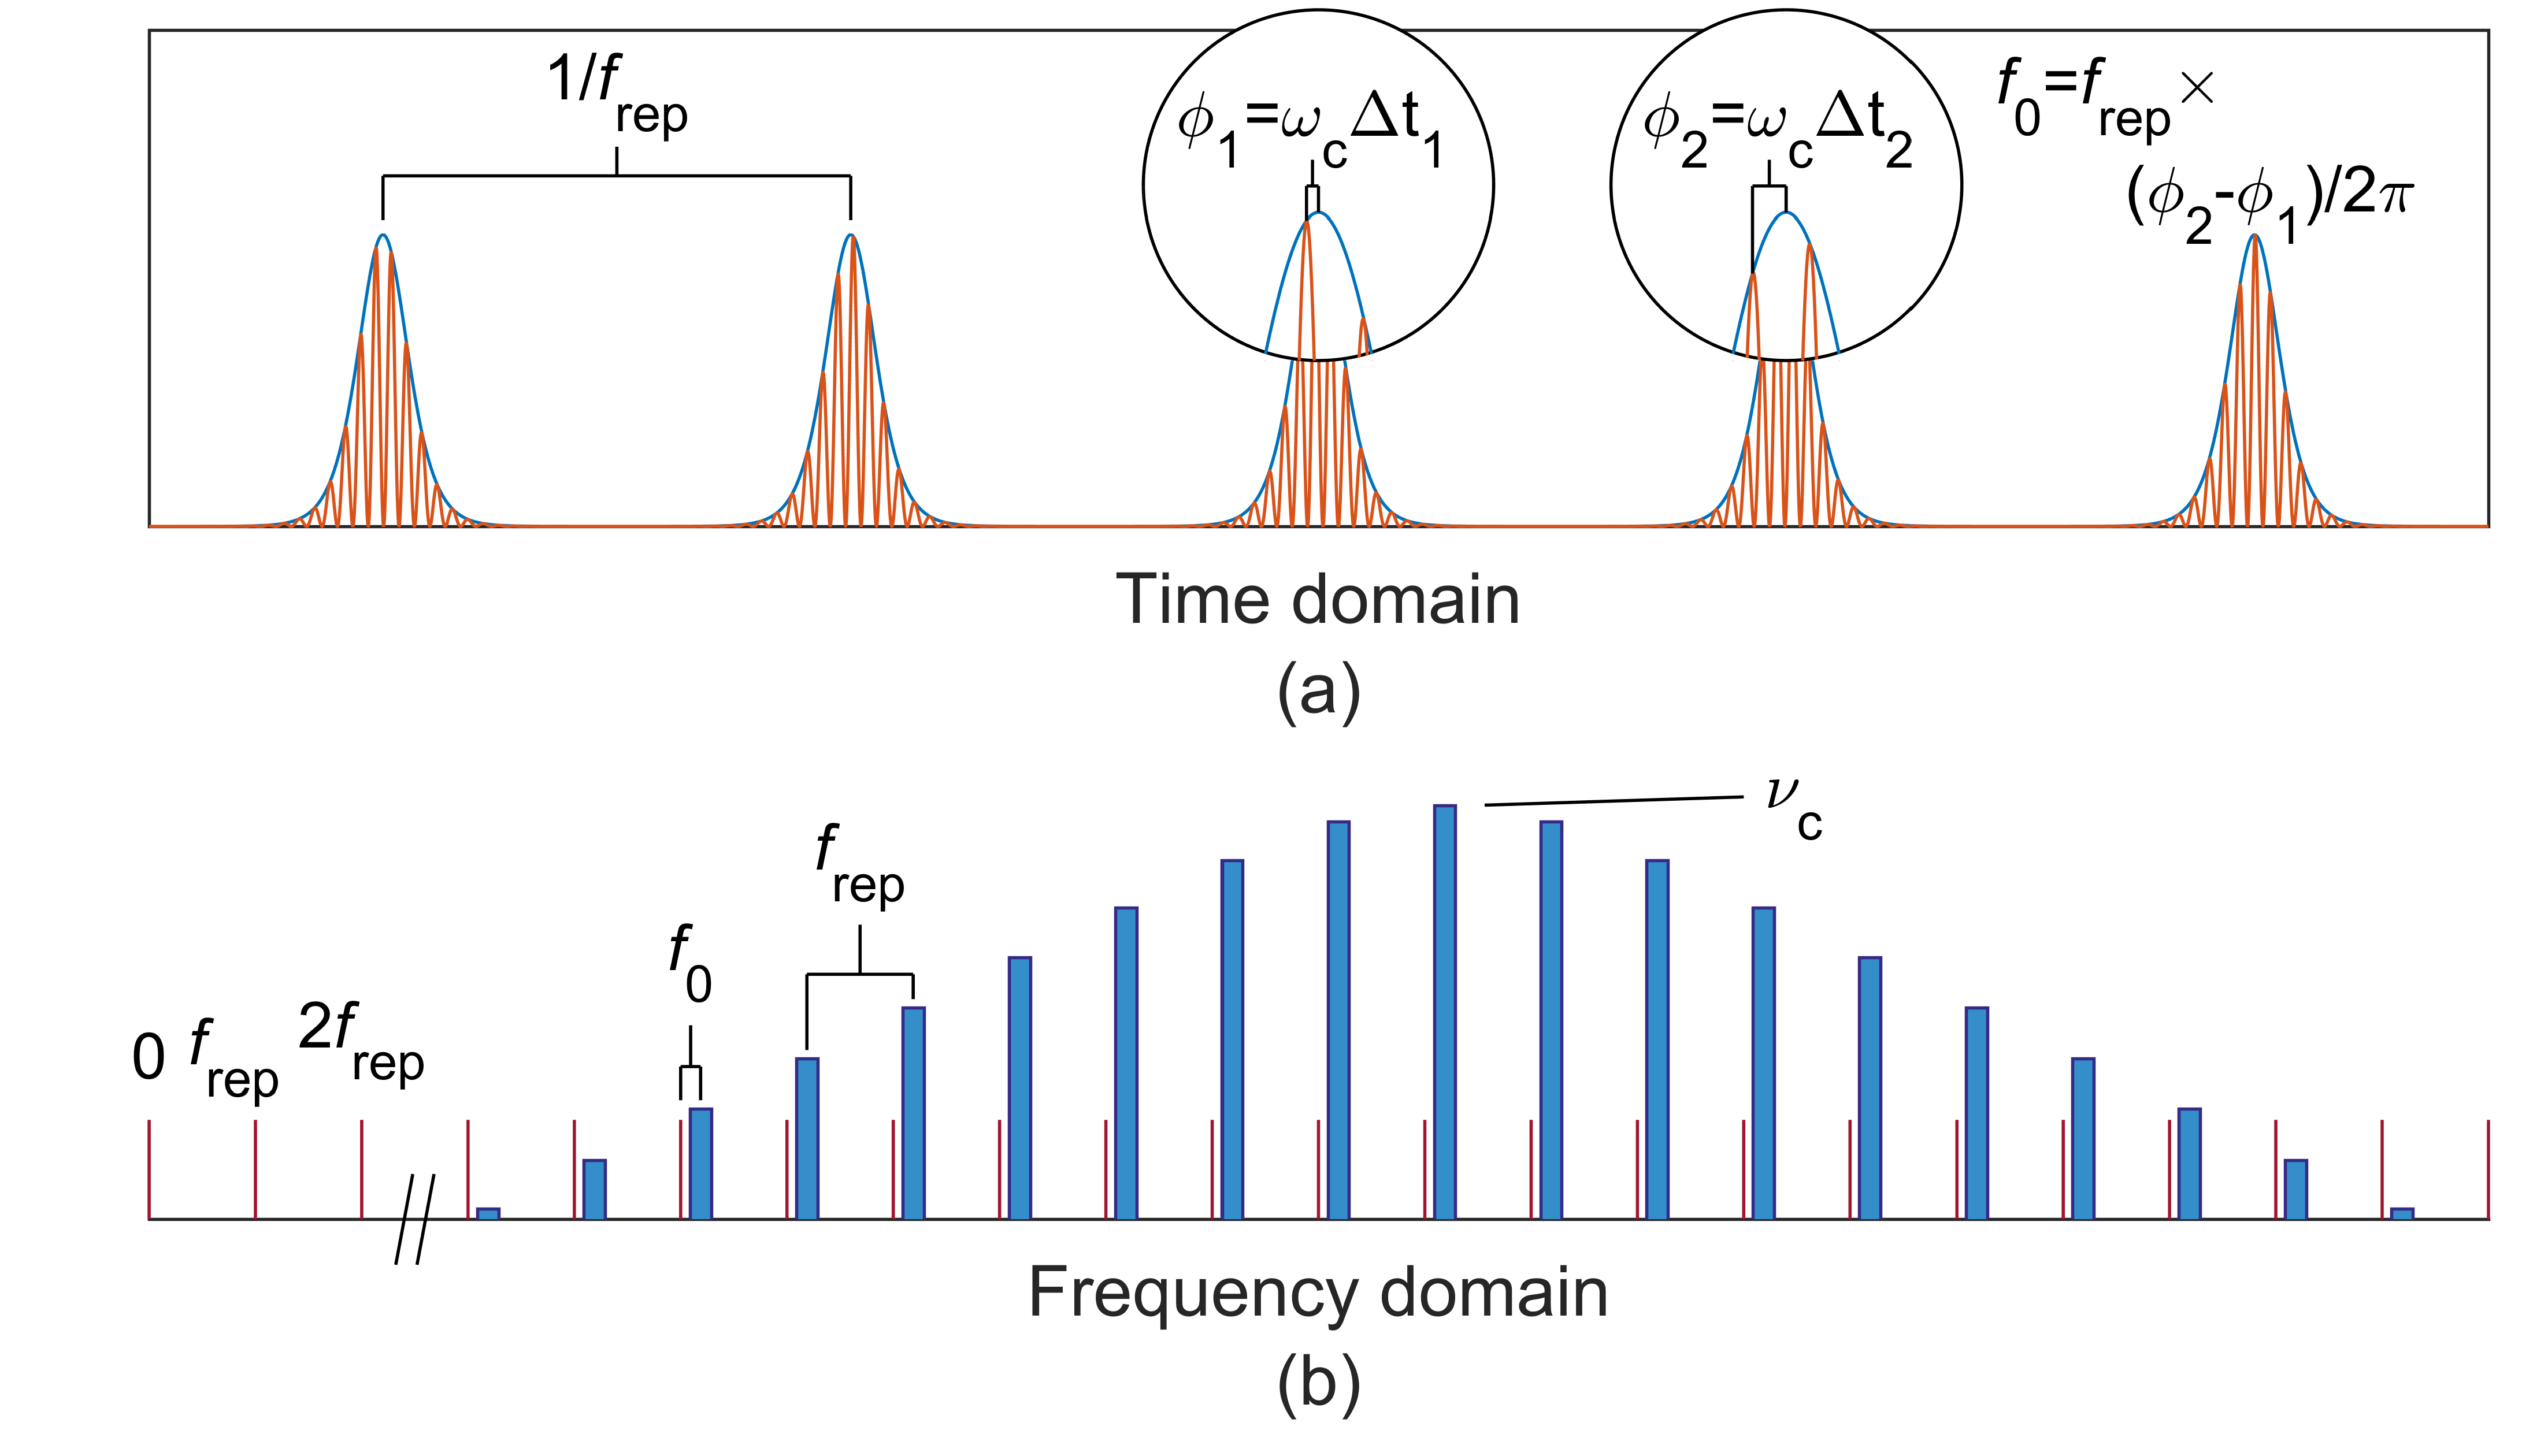
\includegraphics{\FigPath/Figures/Introduction/IntroFCbasics.png}
	\end{center}
	\caption[Optical frequency combs in the time and frequency domains]{\textbf{Optical frequency combs in the time and frequency domains.} (a) Time-domain depiction of a frequency comb as a train of pulses spaced by $1/f_{rep}$. The intensity envelope is shown in blue, and the carrier wave is shown in orange. The carrier-envelope offset frequency $f_0$ arises from a phase-slip of the carrier with respect to the intensity envelope from pulse to pulse. Specifically, if phases $\phi_j=\omega_c\Delta t_j$ are traced out by the carrier wave between its maximum and the $j$\textsuperscript{th} peak of the pulse train, then $f_0=\frac{\phi_{j+1}-\phi_j}{2\pi}f_{rep}$. (b) Frequency-domain depiction of the same frequency comb. The comb modes (shown in blue) are centered around an optical frequency $\nu_c$ and offset from harmonics of the repetition rate $f_{rep}$ (shown in red) by a frequency shift $f_0$. Note that the x-axis has been broken, and the zero-referenced mode numbers of the comb modes shown are large, e.g. $n\sim19340$ for a 10 GHz repetition-rate comb centered at 1550 nm wavelength (see Chapter \ref{chap:EOMCombs}). }
	\label{fig:CombBasics}
\end{figure} 

It is useful to consider a mathematical treatment of an optical pulse train to understand the relationships presented above. In the time domain, the electric field $E(t)$ of the pulse train consists of optical pulses that arrive periodically and have baseband (centered at zero frequency) field envelope $A(t)$ multiplying the carrier wave of angular frequency $\omega_c=2\pi\nu_c$:
\begin{equation}
E(t)=\sum_{k=-\infty}^{\infty} A(t-kT)e^{i\omega_c t}. \label{eq:pulsetrain}
\end{equation}
Here, $T$ is the repetition period of the pulse train. Eq. \ref{eq:pulsetrain} can be viewed as describing a laser of angular frequency $\omega_c$ with a time-varying amplitude. This temporal modulation leads to the distribution of the power across a spectrum whose width scales inversely with the temporal duration of $A$. Intuitively, the spectrum of the comb is the spectrum of the periodic baseband field envelope\footnote{which, as the spectrum of a periodic function, is already a comb.} $\Sigma_k A(t-kT)$, shifted by the multiplication with $e^{i\omega_c t}$ so that it is centered around the optical carrier. More formally, we can calculate the frequency content of the comb by calculating
\begin{equation}
\mathcal{F}\left\{E\right\}(\omega)\sim\left(\sum_{k=-\infty}^{\infty}\mathcal{F}\left\{A(t-kT)\right\}\right)*\delta(\omega-\omega_c),
\end{equation}
which results from the convolution (denoted by $*$) theorem for Fourier transforms; $\mathcal{F}$ denotes Fourier transformation. We use the Fourier transform's property that a temporal translation results in a linear spectral phase shift to obtain:
\begin{equation}
\mathcal{F}\left\{E\right\}\sim\left(\mathcal{F}\left\{A\right\}\times\sum_{k=-\infty}^{\infty}e^{-i\omega kT}\right)*\delta(\omega-\omega_c).
\end{equation}
The quantity $\Sigma_ke^{-i\omega kT}$ is the Fourier-series representation of the series of $\delta$-functions \mbox{$\Sigma_\mu\delta(\omega-2\pi\mu/T)$}, so we have
\begin{equation}
\mathcal{F}\left\{E\right\}(\omega)\sim\left(\mathcal{F}\left\{A\right\}\times\sum_{\mu=-\infty}^{\infty}\delta\left(\omega-2\pi \mu/T\right)\right)*\delta(\omega-\omega_c),
\end{equation}
and performing the convolution leads to the replacement of $\omega$ with $\omega-\omega_c$, leading to:
\begin{equation}
\mathcal{F}\left\{E\right\}\sim\sum_{\mu=-\infty}^{\infty}\delta\left(\omega-\omega_c-\mu\omega_r\right)\mathcal{F}\left\{A\right\}(\omega-\omega_c), \label{eq:combspectrum}
\end{equation}
where $\omega_{rep}=2\pi f_{rep}=2\pi/T$. This expression indicates that the spectrum of the comb has frequency content at modes $\nu_\mu=\nu_c+\mu f_{rep}$, and that their amplitudes are determined by the spectrum of the baseband field envelope, shifted up to the optical carrier frequency $\nu_c$. This is the natural formulation in the case of a comb derived from a CW laser, but it obscures the carrier-envelope offset frequency in the difference between $\nu_c$ and the nearest multiple of the repetition rate, as discussed above. In practice, if $f_{rep}$ is known, then a measurement of $f_0$ is equivalent to a measurement of the frequency of the input CW laser.


\subsection{Frequency stabilization of optical pulse trains}

The scientific need for a method to measure optical frequencies motivated the development of optical frequency combs. While the measurement bandwidth of electronic frequency counters has improved since 1999, it remains limited to frequencies roughly one \textit{million} times lower than the frequency of, e.g., visible red light. Frequency combs present a method for measurement of the unknown frequency $f_{opt}$ of an optical signal through heterodyne with a frequency comb---if $f_{opt}$ falls within the bandwidth of the frequency comb, then the frequency of the heterodyne between the comb and the signal is guaranteed to be less than $f_{rep}/2$, which at least for modelocked-laser-based combs can be measured electronically. Therefore, if the frequencies of the comb are known, measurement of the heterodyne of the comb with the signal reveals the frequency of the signal, provided that the comb mode number and sign of the beat can be determined. This can be done via a wavelength measurement if sufficient precision is available, or by measuring the change $\partial f_b/\partial f_{rep}$, where $f_b$ is the measured frequency of the beat.

The unique utility of the optical frequency comb lies in the fact that measurement of the two microwave frequencies $f_{rep}$ and $f_0$, along with a measurement of the spectral envelope, is sufficient to determine the optical frequencies of all of the modes of the comb, thereby enabling frequency measurement of optical signals. Measurement of the repetition rates of optical pulse trains was possible for many years before the realization of optical frequency comb technology, as this can be done by simply impinging the pulse train on a photodetector. It was the confluence of several technological developments around the turn of the twenty-first century that allowed detection and measurement of the carrier-envelope offset frequency, thereby enabling creation of fully-stabilized modelocked-laser pulse trains: optical frequency combs.

The carrier-envelope offset frequency of a pulse train is challenging to measure because it describes evolution of the optical carrier wave underneath the intensity envelope, and therefore cannot be measured through straightforward detection of the intensity of the pulse train. Presently, the most straightforward way to measure $f_0$ is $f-2f$ \textit{self-referencing}. This can be performed only with a pulse train whose spectrum spans an octave---a factor of two in frequency. Given such an octave-spanning supercontinuum spectrum, a group of modes near mode number $N$ is frequency-doubled in a medium with the $\chi^{(2)}$ nonlinearity \cite{Boyd2003}. This frequency-doubled light is heterodyned with the native light in the supercontinuum with mode number near $2N$. The frequency of the resulting beat $f_b$ is:
\begin{align}
f_b&=f_{doubled}-f_{native}\\
&=2(Nf_{rep}+f_0)-(2Nf_{rep}+f_0)\\
&=f_0.
\end{align}
Such a scheme is typically performed in a `$f-2f$ interferometer,' which is depicted in Fig. \ref{fig:f2f}. Generating the necessary octave-spanning supercontinuum spectrum typically requires nonlinear spectral broadening of the pulse train after its initial generation, except for in specific, carefully engineered cases (e.g. \cite{Fortier2003}). Achieving the required degree of spectral broadening while preserving the coherence properties of the pulse train is a significant challenge---in the past this has typically required launching a train of high energy ($\sim$1 nJ), temporally short ($\leq$ 100 fs) pulses into the spectral-broadening stage. Recent developments in nonlinear waveguide technology have relaxed these requirements slightly (e.g. Ref. \cite{Carlson2017}), but maintaining the coherence of the pulse train during spectral broadening remains one of the important engineering considerations in designing optical frequency comb systems, as discussed in Chapters \ref{chap:EOMCombs} and \ref{chap:PulsePicking}. 

\begin{figure}[htpb]
	\begin{center}
		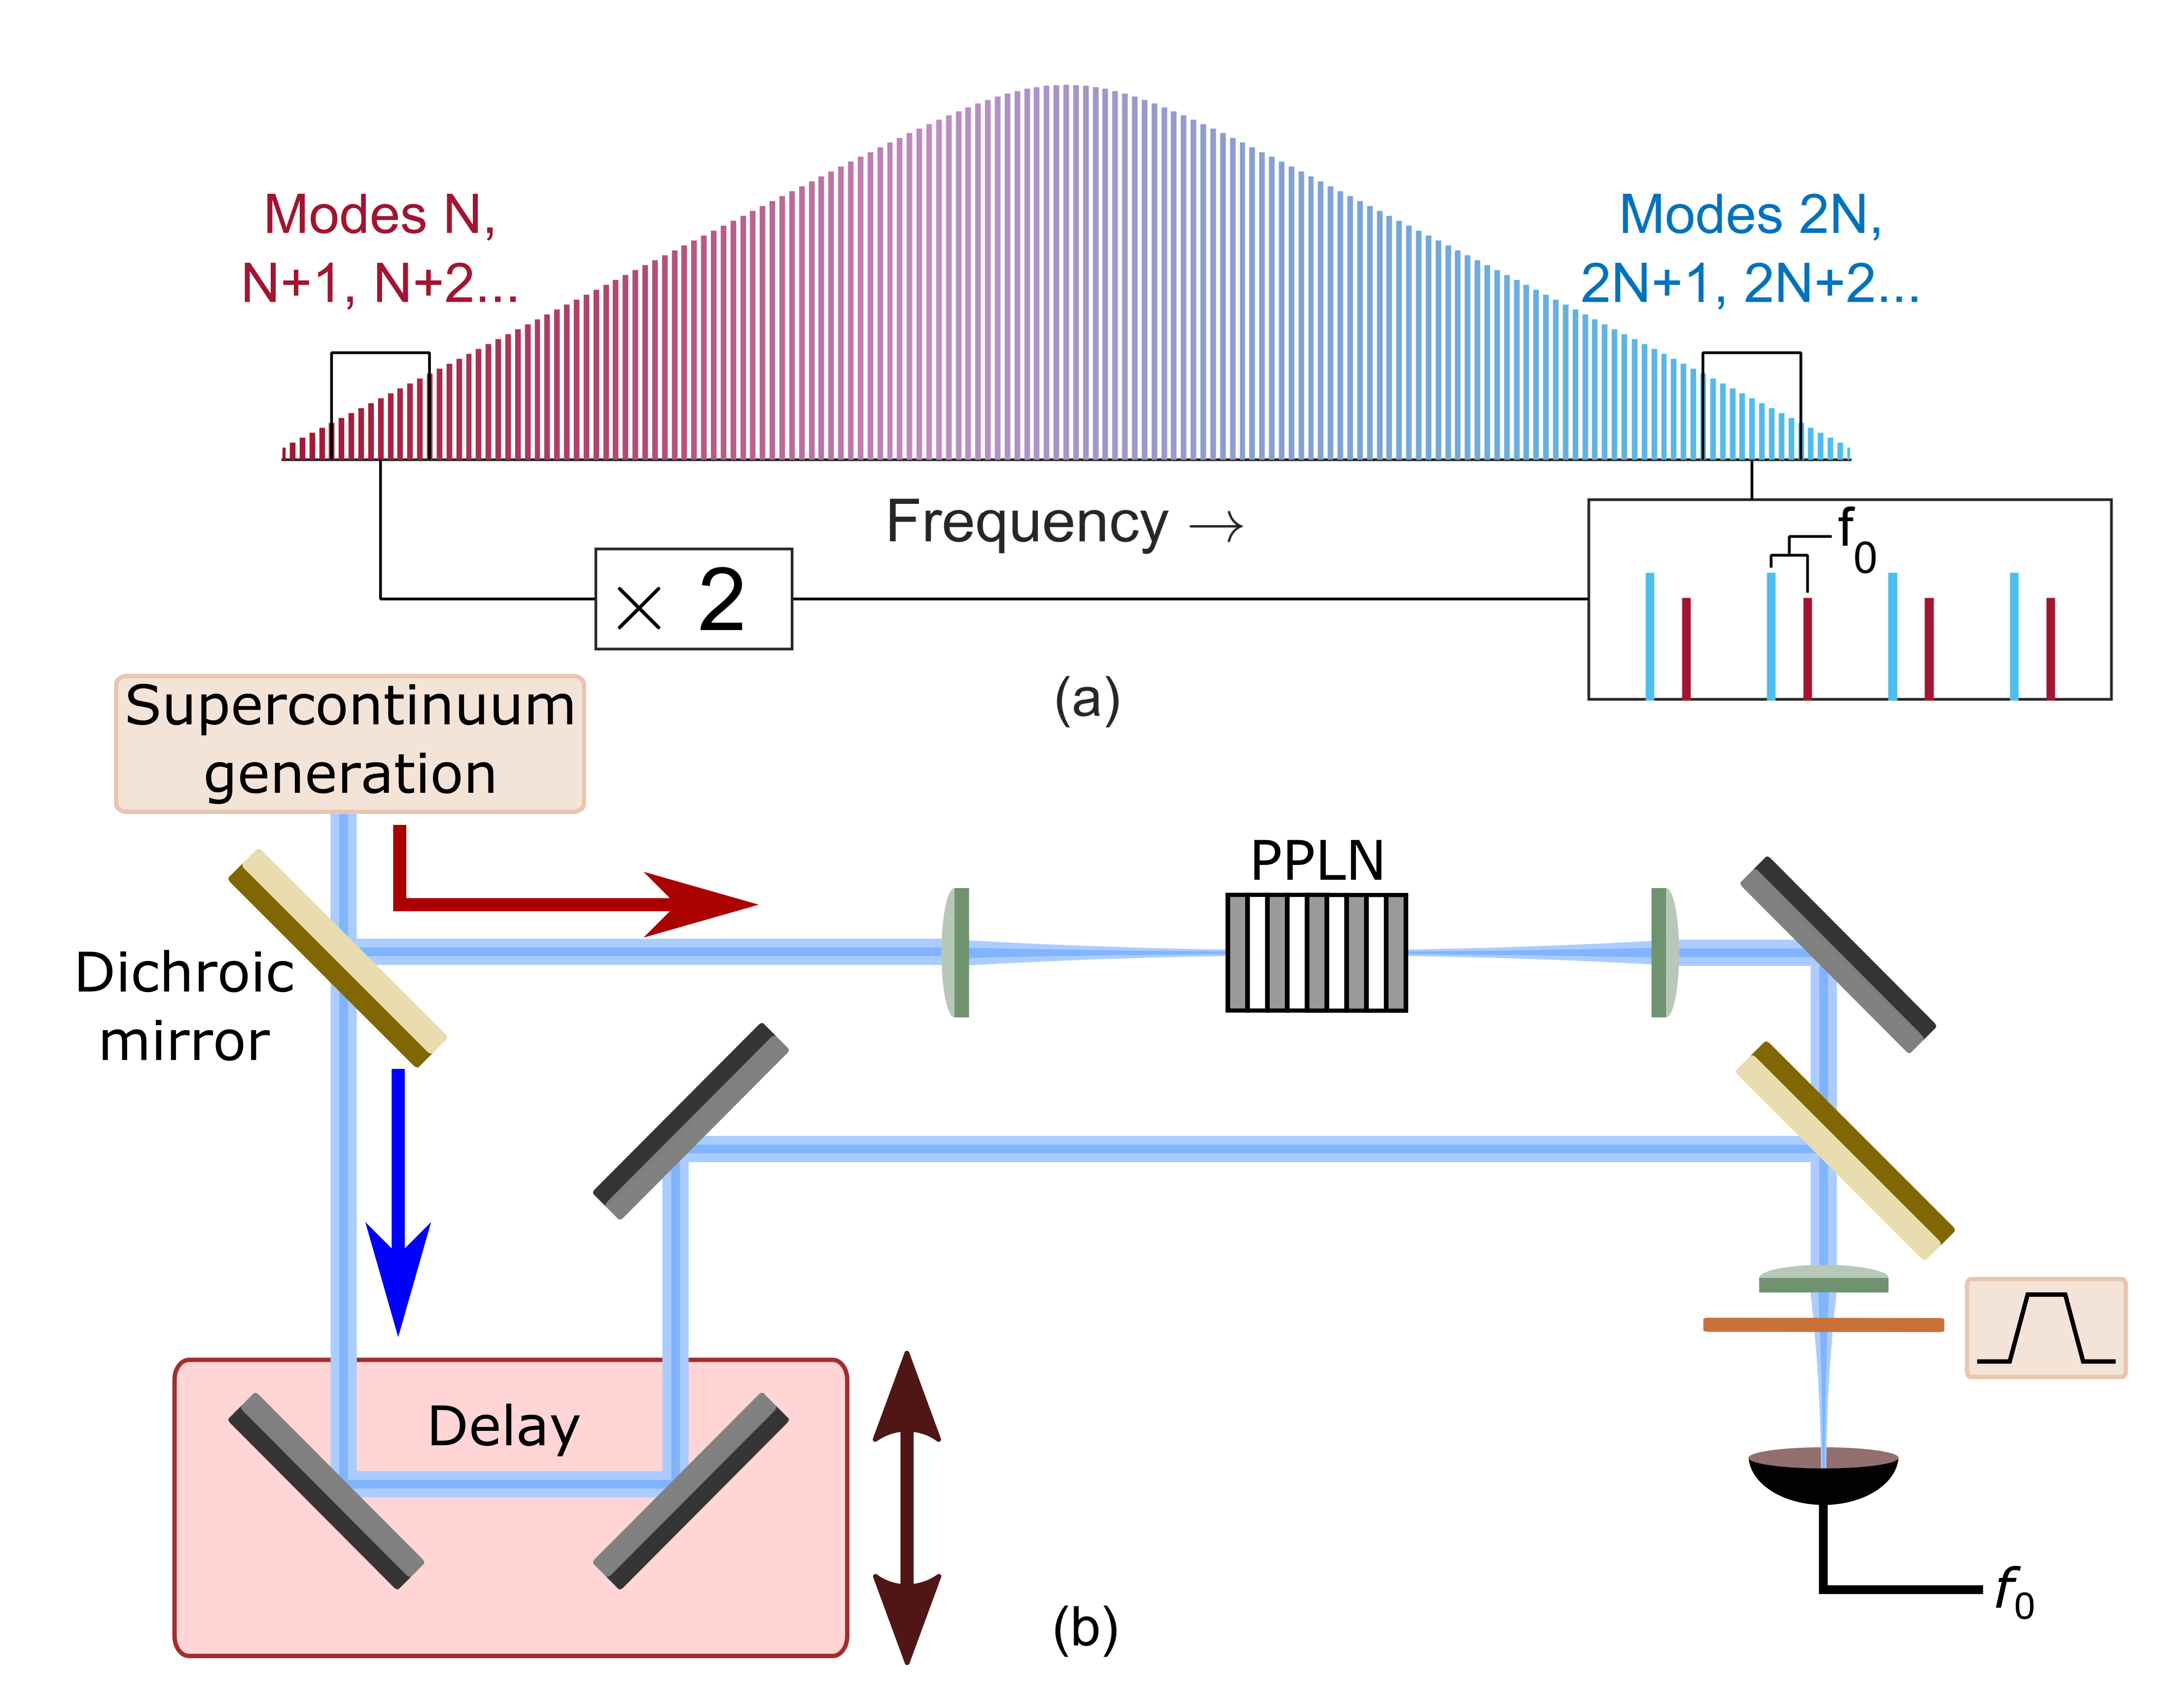
\includegraphics{\FigPath/Figures/Introduction/Introf2fv3.png}
	\end{center}
	\caption[Measurement of the carrier-envelope offset frequency via $f-2f$ self-referencing]{\textbf{Measurement of the carrier-envelope offset frequency $f_0$ via $f-2f$ self-referencing.} (a) Frequency-domain depiction of $f-2f$ self-referencing: Light on the low frequency end of an octave-spanning supercontinuum is frequency-doubled, and then heterodyned with light on the high frequency end near twice its frequency, enabling measurement of the carrier-envelope offset frequency. (b) Schematic depiction of a basic $f-2f$ interferometer: After supercontinuum generation, a dichroic mirror splits the light by wavelength, and the low-frequency end of the supercontinuum is sent (red arrow) through a nonlinear crystal for frequency-doubling. Here the crystal is periodically-poled lithium niobate (PPLN), where quasi-phase-matching is employed for efficient doubling of the target modes. The high-frequency end is sent (blue arrow) through a delay stage, which can be adjusted to compensate for temporal walk-off between spectral the components (modes $\sim N$ and modes $\sim 2N$) required for self-referencing during the supercontinuum-generation process. The paths are then re-combined by a second dichroic mirror and sent through a narrow optical band-pass filter centered around the doubled modes, which filters out unneceessary light and increases the signal-to-noise ratio of the detected $f_0$ signal. Photdetection of the band-passed beam then reveals $f_0$.}
	\label{fig:f2f}
\end{figure} 

%\section{Emerging applications for frequency combs}
%\todo{Here i suppose I'd like to present some example applications}
%The work presented in this thesis is motivated by a set of applications that can leverage high frequency-comb repetition rate; or low frequency-comb size, weight, and power; or both. In general these applications exist outside the laboratory, in fields such as 

%------------------------------------------------------
%
%modes at the set of frequencies 
%
%
%
%Equivalently, if the function $A(t)$ is localized to a small interval around zero relative to the period $T$, this equation be written to emphasize the phase-shift between the carrier wave and the intensity envelope:
%\begin{equation}
%E(t)=\sum_{n=-\infty}^{\infty} A(t-nT)e^{i\omega_c (t-nT)}e^{in\phi_{CE}}, 
%\end{equation}
%where here the field $A(t)e^{i\omega_c t}$ is repeated every period, and is multiplied by a phase increasing incrementally by $\phi_{CE}=\omega_c T$. Eq. 
%
%
%
%\color{red}
%The spectrum of the frequency comb consists of a set of uniformly spaced optical modes at frequencies , multiplied by an overall spectral envelope centered at the optical carrier frequency and corresponding to the temporal intensity envelope of the pulses. The optical frequencies $\nu_n$ are spaced by $f_{rep}$. The carrier-envelope offset frequency $f_0$ represents the offset of the zero\textsuperscript{th} comb mode from zero frequency, and therefore the offset of each mode $\nu_n$ from the closest harmonic of the repetition rate. This offset arises from the pulse-to-pulse evolution of the carrier wave under the pulse train's intensity envelope. 
%
%
%A significant challenge in using $f-2f$ self-referencing to measure the offset frequency of a pulse train is to generate the required octave-spanning supercontinuum spectrum with noise properties that permit detection of the beat between the $f_{doubled}$ and $f_{native}$ signals. In general, this requires nonlinear spectral broadening of the pulse train after its initial generation\todo{except Tara, and others??}, and 
%
%
%In the above, we have used the linearity and convolution properties of the Fourier transform, with convolution denoted by $*$. We have also used the Fourier transform for the Dirac comb . Eq. \ref{eq:combspectrum} directly reveals the connection between the spectrum  of the electric field of a pulse train and the baseband pulse envelope $A(t)$, the carrier frequency $f_c=\omega_c/2\pi$, and the repetition rate $f_{rep}=1/T=\omega_r/2\pi$.
%
%The first optical frequency combs came about through full frequency-stabilization of optical pulse trains generated in modelocked lasers. A laser cavity with broadband gain can support many oscillating frequency modes; this number is on the order of ten thousand for a typical telecommunications-band fiber laser, and can be hundreds of thousands for a Ti:sapphire laser cavity. Without a mechanism to enforce a fixed relationship between the modes, the modes oscillate independently and the laser output is uncontrolled. A modelocked laser is obtained through the introduction of a modelocking mechanism that provides for lower cavity losses in pulsed operation, in which the modes oscillate together and periodically constructively interfere, relative to unsynchronized multi-mode operation. Common modelocking mechanisms are saturable-absorber mirrors, Kerr-lens modelocking, and nonlinear polarization-rotation modelocking.
%
%The pulse train generated in a modelocked laser can be described equally well in either the time domain or the frequency domain. 
%
%
%The spectrum of the pulse train consists of a set of equidistant modes with optical frequencies described by $\nu_n=nf_{rep}+f_0$. Here $\nu_n$ is the frequency of the $n$\textsuperscript{th} mode, referenced to zero frequency; $f_{rep}$ is the pulse train's repetition rate, and is the separation between adjacent modes in the frequency domain, and $f_0$ is the 'carrier-envelope-offset frequency,' denoting 
%
%
%modelocked laser consists of many oscillating modes, supported by broadband laser gain, that have a fixed phase relationship imposed by a modelocking mechanism. In a typical 250 MHz repetition-rate optical pulse train in erbium-doped fiber, this number is on the order of ten thousand.  These pulse trains result from synchronization of many oscillating laser modes in a cavity with broadband gain through the introduction of a modelocking mechanism. A modelocked laser consists of a laser cavity having 1. broadband gain and 2. a modelocking mechanism. generate an optical pulse train when it has broadband gain in the presence of a modelocking mechanism. If a laser is made to oscillate under these conditions without a modelocking mechanism, these modes can 'lase' independently. This generates an output waveform that appears random, resulting from the superposition of these thousands of modes and their individual frequency fluctuations. If, on the other hand, modelocking is enforced so that the modes oscillate in a coherent fashion, their electric field frequency components periodically constructively interfere, yielding a train of pulses. This is depicted schematically in Fig. \cite{fig:MLnoMLpulsetrains}. To induce modelocking, a mechanism that favors higher peak-intensity pulsed operation is introduced into the cavity. Two common modelocking mechanisms are Kerr-lens based modelocking, in which the spatial Kerr effect focuses a  beam through a small aperture in the laser cavity more effectively at higher power, and semiconductor saturable absorber mirrors that have higher reflectivity at higher incident intensities. Modelocking can be used to generate laser pulses that are on the order of hundreds of femtoseconds long, or even shorter.
%\color{black}




